\section{多项式环}

\begin{definition}[多项式环]
    整数环、有理数域、实数域上的全体多项式构成的\textbf{多项式环}:
    \begin{align*}
        \Z[x] = \{\sum_{i=0}^n a_i x^i | a_i \in \Z, n \ge 0\} \\
        \Q[x] = \{\sum_{i=0}^n a_i x^i | a_i \in \Q, n \ge 0\} \\
        \R[x] = \{\sum_{i=0}^n a_i x^i | a_i \in \R, n \ge 0\}
    \end{align*}
\end{definition}

\begin{definition}
    设 \(R\) 是一个整环. 系数取自 \(R\) 的全体多项式构成的集合:
    \begin{equation*}
        R[x]=\{\sum_{i=0}^n a_i x^i | a_i \in R, n \ge 0\}
    \end{equation*}
    则称 \(R[x]\) 是\textbf{多项式整环}.
\end{definition}

\begin{definition}
    设 \(f(x),g(x)\) 是多项式整环 \(R[x]\) 中的任意两个多项式, 其中 \(g(x) \ne 0\).
    如果存在多项式 \(q(x)\) 使得等式 
    \[f(x) = q(x) \cdot g(x)\]
    成立,就称 \(g(x)\) \textbf{整除} \(f(x)\), 记为 \(g(x) \mid f(x)\).
\end{definition}

\begin{definition}[不可约多项式]
    设 \(f(x)\) 是整环 \(R\) 上的非常数多项式. 如果除了平凡因式 \(f(x)\) 以外,
    \(f(x)\) 没有其他非常数多项式, 那么, \(f(x)\) 就称为 \textbf{不可约多项式};
    否则称为可约多项式.
\end{definition}

\textit{例子: \(4x^2+4\) 是一个不可约多项式.}

\begin{theorem}
    设 \(f(x)\) 是域 \(K\) 上的次数为 \(n\) 的可约多项式, \(p(x)\) 是 \(f(x)\) 的
    次数最小的非常数因式. 则 \(p(x)\) 一定是不可约多项式, 且
    \[\deg p < \frac{1}{2}\deg f\]
\end{theorem}

\begin{theorem}
    设 \(f(x)\) 是域 \(K\) 上的多项式, 如果 
    \(\forall p(x)\) 满足 \(\deg p < \frac{1}{2}\deg f\)
    且 \(p(x)\) 不可约, 都有: \(p(x) \nmid f(x)\),
    则 \(f(x)\) 一定是不可约多项式.
\end{theorem}

\begin{example}
    \(f(x) = x^8 + x^4 + x^3 + x + 1\) 是 \(\F_2[x]\) 中的不可约多项式.
\end{example}

\begin{definition}[多项式的Euclid除法]
    给定整环上的多项式 \(f(x),g(x) (\deg f \ge \deg g)\),
    那么可以找到两个多项式 \(q(x), r(x)\) 使得
    \[f(x) = q(x) \cdot g(x) + r(x)\]
    且 \(\deg r < \deg g\).
\end{definition}

\begin{definition}[最大公因式, 最小公倍式]
    设 \(f(x),g(x),d(x)\) 是整环 \(R\) 上的多项式. 称 \(d(x)\) 是
    \(f(x),g(x)\) 的 \textbf{最大公因式}, 如果
    \[d(x) \mid f(x), \quad d(x) \mid g(x)\]
    并且 \(\forall h(x) : h(x) \mid f(x), h(x) \mid g(x)\) 都有 \(h(x) \mid d(x)\).

    称 \(m(x)\) 是 \(f(x),g(x)\) 的 \textbf{最小公倍式}, 如果
    \[f(x) \mid m(x), \quad g(x) \mid m(x)\]
    并且 \(\forall h(x) : f(x) \mid h(x), g(x) \mid h(x)\) 都有 \(m(x) \mid h(x)\).

    \(d(x),m(x)\) 都可以记为 \(\gcd(f(x),g(x)),\lcm(f(x),g(x))\).
\end{definition}

\begin{definition}[多项式互素]
    设 \(f(x),g(x),d(x)\) 是整环 \(R\) 上的多项式.
    若 \(\gcd(f(x), g(x)) = 1\),则称 \(f(x)\) 与 \(g(x)\) 互素.
    记为 \(f(x) \perp g(x)\)
\end{definition}

\begin{theorem}[多项式广义Euclid除法]
    设 \(f(x),g(x),d(x)\) 是域 \(K\) 上的多项式.
    \(\exists s_k(x),t_k(x)\) 使得
    \[s_k(x)f(x) + t_k(x)g(x) = \gcd(f(x),g(x))\]
    对于 \(i = 0,1,2,\cdots,k\). \(s_i(x),t_i(x)\)归纳定义为:
    \[\begin{cases}
        r_{-2}(x) = f(x),\quad r_{-1}(x) = g(x),\quad r_{i} = r_{i-2} \mod{r_{i-1}} \\
        q_{i} = \lfloor \frac{r_{i-2}}{r_{i-1}} \rfloor \\
        s_{-2}(x) = 1,\quad s_{-1}(x) = 0,\quad s_{i}(x) = -q_i(x) s_{i-1}+s_{i-2} \\
        t_{-2}(x) = 0,\quad s_{-1}(x) = 1,\quad t_{i}(x) = -q_i(x) t_{i-1}+t_{i-2} \\
    \end{cases}\]
\end{theorem}

还可以在域 \(K\) 上的多项式环 \(K[x]\) 上完美复刻第二章关于同余的知识点.

\begin{definition}[多项式环的商环]
    设 \(p(x)\) 是域 \(K\) 上的多项式环 \(K[x]\) 中的一个多项式
\end{definition}

\begin{theorem}
    设 \(p(x)\) 是域 \(K\) 上的多项式环 \(K[x]\) 的一个不可约多项式, 
    则 \(K[x]\) 关于理想 \((p(x))\) 的商环 \(K[x]/(p(x))\) 关于
    多项式模 \(p(x)\) 加法以及模 \(p(x)\) 乘法构成一个域.
\end{theorem}
    
\begin{theorem}[有限域构造]
    设素数 \(p\). \(p(x)\) 是多项式环 \(\F_p[x]\) 中
    的一个代数次数为 \(n\) 的不可约多项式, 则 \(\F_p[x]\)
    关于理想 \((p(x))\) 的商环 \(\F_p[x]/(p(x))\) 满足:
    \[\F_p[x]/(p(x)) = \{a_{n-1}x^{n-1} + \cdots + a_1 x + a_0|a_i \in \F_p\}\]
    一般记 \(\F_p[x]/(p(x)) = \F_{p^n}\).
\end{theorem}

\begin{definition}[本原多项式]
    设素数 \(p\). 设 \(f(x)\) 是有限域 \(\F_p\) 上
    的多项式环 \(\F_p[x]\) 中的一个 \(n\) 次多项式. 使得
    \[x^e \equiv 1 \pmod{f(x)}\]
    成立的最小正整数 \(e\) 叫做 \(f(x)\) 在有限域 \(\F_p\)
    上的指数. 记为 \(\ord{p}{f(x)}\).

    特别地, 如果 \(\ord{p}{f(x)} = p^n - 1\), 则称 \(f(x)\)
    为 \(\F_p\) 上的本原多项式
\end{definition}

\begin{example}
    对于计算机最喜欢的 \(\F_2 = (\{0,1\},+_2, (\cdot)_2)\),
    有一个本原多项式 \(x^8+x^4+x^3+x^2+x\), 令
    \[\F_{2^8} = \F_2[x]/(x^8+x^4+x^3+x^2+x)\]
\end{example}

\(\F\) 的本原元就是 \(\F^*\) 的生成元.

\begin{theorem}[\textbf{本原多项式的性质}]
    设素数 \(p\), 设 \(f(x),g(x)\in \F_p[x]\). 则有以下性质:
    \begin{itemize}
        \item 若整数 \(x^d\) 使得 \(x^d \equiv 1 \pmod{f(x)}\), 则 \(\ord{p}{f(x)} \mid d\).
        \item 若 \(g(x) \mid f(x)\), 则 \(\ord{p}{g(x)} \mid \ord{p}{f(x)}\).
        \item 如果 \(\gcd(f(x),g(x)) = 1\), 则 \(\ord{p}{f(x)\cdot g(x)} = \lcm(\ord{p}{f(x)}, \ord{p}{g(x)})\).
        \item 如果 \(f(x)\) 是不可约多项式, 则 \(\ord{p}{f(x)} \mid p^n - 1\).
        \item \(f(x)\) 是本原多项式 \(\implies f(x)\) 是不可约多项式.
    \end{itemize}
\end{theorem}

\begin{theorem}[\textbf{本原多项式判定}]
    设素数 \(p\). 设 \(f(x) \in \F_p[x], \deg f = n\).
    如果 \(x^{p^n - 1} \equiv 1 \pmod{f(x)}\), 且对于
    \(p^n - 1\) 的所有不同素因数 \(q_i\), 都有
    \[x^{\frac{p^n - 1}{q_i}} \ne 1 \pmod{f(x)}\]
    则 \(f(x)\) 是本原多项式.
\end{theorem}

% This file was created with tikzplotlib v0.10.1.
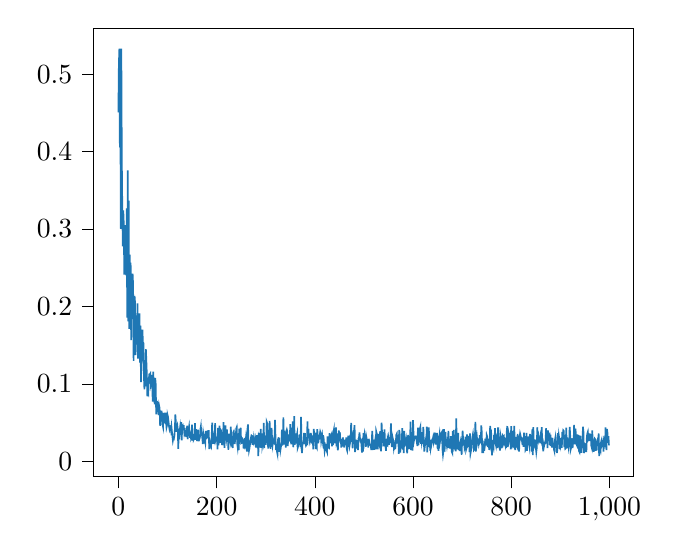
\begin{tikzpicture}

\definecolor{darkgray176}{RGB}{176,176,176}
\definecolor{steelblue31119180}{RGB}{31,119,180}

\begin{axis}[
tick align=outside,
tick pos=left,
x grid style={darkgray176},
xmin=-49.95, xmax=1048.95,
xtick style={color=black},
y grid style={darkgray176},
ymin=-0.0197277497777307, ymax=0.559415687734783,
ytick style={color=black}
]
\addplot [semithick, steelblue31119180]
table {%
0 0.450844607167757
1 0.512305752408677
2 0.533043577927657
3 0.405558400897062
4 0.462659178802355
5 0.300110118435032
6 0.533090986029668
7 0.389196883466339
8 0.324605305092994
9 0.277555827049142
10 0.324228609307864
11 0.307099452888606
12 0.241152647084631
13 0.304883770858823
14 0.293175150804288
15 0.280586930832201
16 0.240021990054056
17 0.326828936626389
18 0.185701881512933
19 0.375730710368401
20 0.180793236991018
21 0.33657917751374
22 0.171044700330549
23 0.26692562953634
24 0.219758215187864
25 0.256485234188923
26 0.156624838589237
27 0.223790250552029
28 0.2000797937005
29 0.242514522464577
30 0.228026866291142
31 0.129557688190514
32 0.197674211745211
33 0.21351671094461
34 0.204727057639929
35 0.137223684376932
36 0.155891984510451
37 0.155375672009551
38 0.165490524731658
39 0.204105878555999
40 0.132708960018502
41 0.169554597945404
42 0.135585126167496
43 0.191191586441534
44 0.127355821292086
45 0.175238551579573
46 0.102136952364581
47 0.128483042245202
48 0.130035565961557
49 0.170131825542691
50 0.151976160687171
51 0.152330670695449
52 0.10963480779561
53 0.0930601742657634
54 0.126825532309632
55 0.0966347206279486
56 0.14497468732278
57 0.129352615795343
58 0.111304449027317
59 0.0838128743650456
60 0.0902343628198851
61 0.0883322151705462
62 0.105645850136294
63 0.112343683408507
64 0.112202132519631
65 0.113265279505192
66 0.100633678042905
67 0.104642477057642
68 0.111457659735733
69 0.0962378066521753
70 0.0769490082849772
71 0.115638136871157
72 0.0974918533915491
73 0.080288814044062
74 0.0735062633543476
75 0.107618814618256
76 0.100127292901274
77 0.0607540603225419
78 0.0771030285065634
79 0.0769253765136644
80 0.073433456607137
81 0.0658768713669941
82 0.0597741719954165
83 0.0716064882670019
84 0.0684823979528936
85 0.045756001926649
86 0.0548776622740779
87 0.0542228576488282
88 0.0653344950725367
89 0.0561713182302177
90 0.0473282912507516
91 0.044235079089268
92 0.0625834222481977
93 0.0572052403835357
94 0.0510545590744013
95 0.0502970278811377
96 0.0627182997731188
97 0.0522273014080906
98 0.0437751551089278
99 0.0465325844968092
100 0.0601981252314483
101 0.0576265575992999
102 0.0518828448542807
103 0.0459068348598076
104 0.0420403898542937
105 0.0454411500631374
106 0.045154138354868
107 0.040583264493228
108 0.0452711313504608
109 0.0383844548446099
110 0.0326067383523746
111 0.0268182013712427
112 0.0301888206707114
113 0.0292265302852192
114 0.0325427968346256
115 0.0409814403013386
116 0.0603998583334404
117 0.050866478113077
118 0.038118236977363
119 0.0450547963057921
120 0.0467925356239194
121 0.0403413508492731
122 0.0161839970398054
123 0.0420681528417968
124 0.0284171410213045
125 0.0400374502796925
126 0.0454135195852304
127 0.0402231747041188
128 0.0506300955220111
129 0.0270336443778359
130 0.0457334416180259
131 0.0464862790108637
132 0.0398765664729795
133 0.0465358604929354
134 0.038633028861771
135 0.0432020432911498
136 0.0322437859515966
137 0.0401822911047509
138 0.0328248600837632
139 0.0331693199640879
140 0.0458802406208291
141 0.0285213459666198
142 0.0353327928714439
143 0.0409196479972983
144 0.0449764934442589
145 0.0370831758864959
146 0.0304267406572807
147 0.0381134744018752
148 0.0293682144526502
149 0.0310328809513865
150 0.0474053246884211
151 0.0267082099411508
152 0.0353281750613572
153 0.0275902487020723
154 0.029009478748653
155 0.0295518955292886
156 0.0491401389318597
157 0.027729748629728
158 0.0413802948074418
159 0.0371122533956795
160 0.0261035377664189
161 0.0327802928537136
162 0.040918906550856
163 0.0268508518185705
164 0.0267979727311001
165 0.0286078958605399
166 0.0308058119655036
167 0.0412178214138261
168 0.0450458283096179
169 0.0350931331454602
170 0.035466227826805
171 0.0295106112558259
172 0.0221571675055882
173 0.0359064768588388
174 0.0318564215073555
175 0.0227601141723537
176 0.0279588170861756
177 0.0242175902824489
178 0.0391465148323246
179 0.0286235161661889
180 0.0340202303534536
181 0.0331754089249999
182 0.0398987052682946
183 0.0296396921301698
184 0.0401397740433203
185 0.0157323881773088
186 0.0228410262182397
187 0.0205014087560023
188 0.0241553560081541
189 0.0213519706270931
190 0.0324503036304831
191 0.0500291181010292
192 0.0287318161004058
193 0.0225705833644568
194 0.03091141698617
195 0.0272344795924163
196 0.0222118206277335
197 0.0491791029385138
198 0.0278505144916438
199 0.0303767893809474
200 0.0276324980829459
201 0.028128713740304
202 0.0155486386380742
203 0.0429918091174397
204 0.0206426790166789
205 0.0315486375904995
206 0.0459440690484644
207 0.0236936480254848
208 0.0410338482576757
209 0.0400099679774999
210 0.0338908640161113
211 0.0208139555372664
212 0.0268440588764953
213 0.0215397756179261
214 0.0504864013300573
215 0.0292538997676242
216 0.017450282663162
217 0.0296522450435712
218 0.0462295914622581
219 0.0347632300280571
220 0.0304148836875513
221 0.0413118832031874
222 0.0277859947137202
223 0.0339545664161068
224 0.0146436701208648
225 0.0355831554203068
226 0.0276081691281051
227 0.0274685394196081
228 0.0247643157782604
229 0.0446277552076326
230 0.0217184987491717
231 0.0206108840884687
232 0.0326229711027826
233 0.0171907271080675
234 0.0374319090040043
235 0.03862336377487
236 0.0315181671508272
237 0.0222945456098542
238 0.0302500318601553
239 0.0298334671625146
240 0.0424611229775988
241 0.0440909655475451
242 0.0232171129254688
243 0.0180889899731141
244 0.0256186540851513
245 0.0144825841580384
246 0.0421291714328269
247 0.028109223205517
248 0.0316470893168643
249 0.0435154461513232
250 0.0233464643417045
251 0.023797361269058
252 0.0264745820972524
253 0.028730682709097
254 0.0275448225764882
255 0.0165582279532557
256 0.021863722411731
257 0.0197698495797131
258 0.0300670654443864
259 0.0250407874456209
260 0.0313929565816146
261 0.0268593031860466
262 0.0123757933368488
263 0.0422526824278875
264 0.0475919058859447
265 0.0231428259635635
266 0.0137701146434464
267 0.0170415939673172
268 0.0213763421383194
269 0.0258131489989729
270 0.0303717648333219
271 0.0333745552699827
272 0.0328798963160028
273 0.0211692616720202
274 0.0261824033978282
275 0.0243397385262755
276 0.0308171140379104
277 0.0270307285325626
278 0.0246658089574984
279 0.0279524110689805
280 0.0176845750670974
281 0.0247404311757327
282 0.0338679234804152
283 0.025209536380847
284 0.0286878742857554
285 0.00659695192738357
286 0.0367355637128532
287 0.0287662754386947
288 0.017664848713036
289 0.0290605167189651
290 0.041752760339158
291 0.0173344433388947
292 0.0361553076700873
293 0.020318353947249
294 0.0242308377914864
295 0.0219377116202105
296 0.0497377777085991
297 0.0170017403250641
298 0.0323095360480945
299 0.0316720215687955
300 0.0212808607301081
301 0.0259478141995722
302 0.0510481464789081
303 0.0492909132520583
304 0.0320732967435045
305 0.0164125013608671
306 0.0330759635795929
307 0.0190332954166819
308 0.0520741028233179
309 0.0257143860331022
310 0.0161413465485787
311 0.037134582908781
312 0.0431726571830688
313 0.0276860540284326
314 0.0212132609879998
315 0.0265008808145677
316 0.0229622373701036
317 0.0229865911100207
318 0.022640676090347
319 0.0534005765691454
320 0.0301547772838685
321 0.0144841165567747
322 0.0210150948948092
323 0.0125768048304241
324 0.00943192167771996
325 0.0282182481908511
326 0.0299279817227895
327 0.0296881078185774
328 0.0122023442982656
329 0.0228112142733225
330 0.0144455944732292
331 0.0185599259297065
332 0.0254606117147781
333 0.0409379326343778
334 0.0203308846292186
335 0.0293258404844399
336 0.0567004863871017
337 0.0295591430330635
338 0.0216575602535702
339 0.0361262208892701
340 0.0347664575257985
341 0.0176914333554072
342 0.0390570882552754
343 0.0410532377663507
344 0.0385704756994921
345 0.019537314648277
346 0.0345491095888459
347 0.0278853020409207
348 0.0270041941285722
349 0.0266253356189868
350 0.0479011038272388
351 0.0275264581652865
352 0.0219962869899369
353 0.0427020639845508
354 0.0236368361667235
355 0.0514324143935987
356 0.0181994936930274
357 0.0240941828962466
358 0.0582191210770702
359 0.0213869494838419
360 0.0302580748018887
361 0.0361110336276828
362 0.022838370113756
363 0.0317736122798342
364 0.035392878086076
365 0.017100145294476
366 0.0190887396226286
367 0.0236316763575916
368 0.0260501725622671
369 0.034767098384159
370 0.0245108276758169
371 0.0182654431087592
372 0.0572217450820607
373 0.0163589760791577
374 0.0105842153449672
375 0.0236488623970802
376 0.0232928926971931
377 0.0233537916125593
378 0.0365374634758213
379 0.0222142194860199
380 0.0362727310141699
381 0.0226605010910609
382 0.020305312879163
383 0.0216701399130381
384 0.0217283919354443
385 0.051420036019824
386 0.0313404788211786
387 0.0416469418772097
388 0.0318643484725722
389 0.0253664111350512
390 0.0279826492241641
391 0.02668546394668
392 0.0366095268689915
393 0.0247757364670406
394 0.0257517626747372
395 0.0332388075305475
396 0.0252780742240578
397 0.0153783444757713
398 0.0417070516921579
399 0.0293908475423836
400 0.0313031387142576
401 0.0368426253330046
402 0.0158070658137261
403 0.0205064774088654
404 0.0185158520128672
405 0.0414387585293854
406 0.0326318998182731
407 0.0231140708324157
408 0.0292091733635927
409 0.0290843745316462
410 0.0336453838605477
411 0.0380181094738298
412 0.0358316433528546
413 0.026078390608682
414 0.0300303448561319
415 0.0338623778195532
416 0.0277935988093487
417 0.0337383179052335
418 0.0165186736208989
419 0.0214148148183788
420 0.0131549652343172
421 0.0170974619238114
422 0.0195913567040524
423 0.0159752889219282
424 0.013957797301211
425 0.0120449648526075
426 0.0322203643531919
427 0.0201312496339435
428 0.018101138965328
429 0.0175008650275967
430 0.036167585105347
431 0.02677413718202
432 0.025807340420067
433 0.032369832166735
434 0.0342776897630153
435 0.0191833360165754
436 0.0286648648443611
437 0.0208732104606667
438 0.0379730390753499
439 0.0411863083428792
440 0.0232738491410407
441 0.0421494492787193
442 0.0336765109169661
443 0.0438831553090298
444 0.025841654261145
445 0.0287710116712777
446 0.0203306110184922
447 0.0141318935027294
448 0.0328520406344199
449 0.0397196084238338
450 0.0271008803488266
451 0.0375943806566073
452 0.0257508805309104
453 0.0263114201069556
454 0.0177801510291968
455 0.0283612098844843
456 0.0188471647551483
457 0.0309345878413935
458 0.025524679939228
459 0.022937655236989
460 0.0178877710247257
461 0.0279486672313719
462 0.0227348580631528
463 0.0230919112917109
464 0.0307482085321015
465 0.0158974196487135
466 0.0135597593865661
467 0.0191581434260705
468 0.0331183647752526
469 0.0284264611382609
470 0.0298358781073492
471 0.0209443904389798
472 0.0248234610127403
473 0.0277917286455618
474 0.0495402398104154
475 0.0318637032023402
476 0.0307148772121793
477 0.0166094460105983
478 0.0260129473710576
479 0.0379821874989001
480 0.0402444852732737
481 0.0466670927529985
482 0.0117769880518633
483 0.0202328950941112
484 0.0279161582359541
485 0.0164006355766106
486 0.0229184444626115
487 0.0271999955530427
488 0.0143064284338062
489 0.0294812084209086
490 0.0308578608634964
491 0.0371336760803572
492 0.0294580370667593
493 0.0260242452677442
494 0.026602236284095
495 0.0213124386862651
496 0.0113155806043036
497 0.0298768015904882
498 0.012551219062626
499 0.0362636300127839
500 0.0315253068226862
501 0.0349666782366396
502 0.0266098575922384
503 0.0315718948461883
504 0.0187130830398922
505 0.0310329789926522
506 0.0276079273388313
507 0.0227922458714801
508 0.0234947347511953
509 0.0178675067179254
510 0.0290155106189811
511 0.023672962182727
512 0.0213791147092758
513 0.0211581227520248
514 0.0200811743035621
515 0.0145413523741984
516 0.0259653296346705
517 0.0393586936213369
518 0.0227974579558747
519 0.0146326092392296
520 0.0277829075730201
521 0.0146934864097232
522 0.0230487547987446
523 0.0272446005598616
524 0.0155027723567442
525 0.0387379827668396
526 0.0360654045706116
527 0.0284075655754105
528 0.01543384668682
529 0.0230033113740284
530 0.035413398061556
531 0.021875380605017
532 0.0198079973277488
533 0.0389703654696343
534 0.0186843383918967
535 0.0129523429865925
536 0.0500127968925589
537 0.0355216477886254
538 0.0359258959008264
539 0.0290066928501697
540 0.0191777582258014
541 0.0292437865936175
542 0.0411158014758968
543 0.0212991535303144
544 0.0186130149757231
545 0.0136416789072657
546 0.0289899160101011
547 0.019164794735004
548 0.028093319372185
549 0.0245315353517076
550 0.0290518652762337
551 0.021335262872178
552 0.0305387868057842
553 0.0306180269619644
554 0.0235261047138735
555 0.0489587138811811
556 0.0257903809449142
557 0.0182168461954314
558 0.0319111239192333
559 0.0289348488451977
560 0.02604204115415
561 0.0172001035902417
562 0.0207556681174632
563 0.0163850756117399
564 0.0167816841444074
565 0.0251985252819802
566 0.0341865269018988
567 0.0355670368794668
568 0.0229900687837846
569 0.0311561746400422
570 0.0324607641304996
571 0.00947758480223057
572 0.0404624228926725
573 0.0341304058910024
574 0.0113078290381425
575 0.0198300669694402
576 0.0199952445780023
577 0.0188511098125305
578 0.0426580641893172
579 0.0313217176806618
580 0.0272213026852286
581 0.0106799084770933
582 0.0392552680195959
583 0.0204427511671181
584 0.0216259012551293
585 0.0248514998575719
586 0.0291089310056356
587 0.0240375225789933
588 0.0104221048948069
589 0.0184729794225391
590 0.0342013347309116
591 0.0229742365966063
592 0.0226722960095504
593 0.0157438013956237
594 0.029965954321541
595 0.0510807144950888
596 0.0145808079250219
597 0.0352777513065018
598 0.0190488667138752
599 0.0137639426460074
600 0.0532845098958559
601 0.0356101502921259
602 0.0269523411585524
603 0.0306822166423382
604 0.0312495237458076
605 0.0322198213833301
606 0.0321844982039638
607 0.0279783768881308
608 0.0325448133652914
609 0.0196273413381273
610 0.0433183561426412
611 0.021067850540653
612 0.0267499624706642
613 0.028637899841948
614 0.0420234226892414
615 0.0444049268560647
616 0.02259782543135
617 0.0375768883101516
618 0.0254534438317889
619 0.0296116908208682
620 0.0225186638832014
621 0.0444051635810831
622 0.0247798985054822
623 0.0126215334242731
624 0.0191013853346835
625 0.0235367171708432
626 0.0276179815463825
627 0.0211215226770717
628 0.0448464172437733
629 0.0116361580155178
630 0.0277025106176855
631 0.0186772010591599
632 0.0437316423562539
633 0.0303658202952783
634 0.0230327964437102
635 0.0277321369101871
636 0.0163539523454535
637 0.0196707137141764
638 0.0229776379348348
639 0.0278778719743953
640 0.0276550482209038
641 0.0309715317353023
642 0.0254523344533392
643 0.0295381047158793
644 0.0242668577589154
645 0.0369055866222146
646 0.0216477639454252
647 0.0363159386220328
648 0.0279585578035012
649 0.0366633425554063
650 0.0173648099928257
651 0.0175578996298863
652 0.013616154456485
653 0.0301539550183585
654 0.0347216186338997
655 0.0255477330043011
656 0.0294218437998771
657 0.0336845114803065
658 0.0368846822775361
659 0.0379712314609689
660 0.0152411433962113
661 0.00859151434233018
662 0.013732519196491
663 0.0414279527964514
664 0.0123790357935623
665 0.0200691123486719
666 0.0380554557327539
667 0.0251787211558027
668 0.0242086646624998
669 0.0198791039656573
670 0.0247097184043667
671 0.0169389307610023
672 0.039151126791674
673 0.0220638408024865
674 0.02782277265006
675 0.016543326698544
676 0.0250801325930109
677 0.0325251664135255
678 0.0190667455658986
679 0.0122290083441097
680 0.0107197944848897
681 0.0390403898277889
682 0.0210850687954095
683 0.0406775906437203
684 0.018335672875877
685 0.0203291767159719
686 0.0337675638801909
687 0.0129712810238793
688 0.0554652623237518
689 0.0217692129776305
690 0.0238244677808149
691 0.0155553316021453
692 0.036519218155482
693 0.0144446656901507
694 0.0209482993311033
695 0.0131860949139412
696 0.0214307812437845
697 0.0252197447186512
698 0.0207266663836769
699 0.00847239870672688
700 0.02763007650597
701 0.0394302085786084
702 0.0284416793207026
703 0.020239441121689
704 0.0278992216609059
705 0.0168453956836708
706 0.0188914737378013
707 0.0318346695064786
708 0.0147248650340647
709 0.016957055867324
710 0.0347866739191867
711 0.0241285553615531
712 0.0203180677672602
713 0.021367860143082
714 0.0328944291546479
715 0.0118473747414432
716 0.0359468929697538
717 0.0102321407612497
718 0.0136514965334115
719 0.0169830919715027
720 0.026770044959135
721 0.0314236216379537
722 0.0349815472816272
723 0.0273145299980455
724 0.0143744928045978
725 0.0152206642273739
726 0.0294746632486287
727 0.0509172856200563
728 0.0125076104629103
729 0.0272451594412397
730 0.0316032188093001
731 0.0248153788221423
732 0.0282192722613135
733 0.0275772229575951
734 0.0225604807034633
735 0.0260566530354459
736 0.0336369531665115
737 0.0245606562677436
738 0.0253357033479203
739 0.0464476938363863
740 0.0374901971458618
741 0.0107162035997944
742 0.0265251491353841
743 0.0105050151018867
744 0.0227962930639485
745 0.0134286418699842
746 0.0184560701936101
747 0.0281223038867197
748 0.0280333656312784
749 0.0202044973846781
750 0.0340033477238347
751 0.0321272719361669
752 0.0182783218285684
753 0.0262293362465396
754 0.0271631107523513
755 0.0156413034675491
756 0.0155041300222693
757 0.0456112596619879
758 0.0393345722106199
759 0.0394506051392036
760 0.0155842317391588
761 0.00759454768216699
762 0.0276757187842681
763 0.0213732729219656
764 0.0186512468223053
765 0.0341986990558583
766 0.0280212649650558
767 0.0426620794197241
768 0.0236852205738624
769 0.0203723281174762
770 0.0271868906626291
771 0.0230346157075554
772 0.0170176616588856
773 0.0438130232198967
774 0.0242511326904556
775 0.031777829665634
776 0.0198890773177325
777 0.0139277115475264
778 0.0343815397084326
779 0.0311292188472526
780 0.0166331237522102
781 0.0330763458492319
782 0.0177429526395789
783 0.0326133725385732
784 0.0314206272340903
785 0.0322904113183802
786 0.0219272855239242
787 0.0222005314379422
788 0.0199769023647611
789 0.0305336432443126
790 0.0172438423355899
791 0.0394384335071857
792 0.0454881598200585
793 0.0185590966675405
794 0.0225759634121748
795 0.0332089136809343
796 0.0288614749464178
797 0.0312851471113681
798 0.0344370768053276
799 0.0155344308565728
800 0.0454568035212661
801 0.0165559230483302
802 0.0391759347398832
803 0.0260090848096108
804 0.0203549601863231
805 0.0192195416588532
806 0.0456109415337286
807 0.0293724383103183
808 0.0143386839282287
809 0.0313800276769297
810 0.0231445448750757
811 0.0198583558558195
812 0.0187436104893343
813 0.0352785426870221
814 0.0142531386585066
815 0.0211637927144991
816 0.0126451541402926
817 0.0305022313799769
818 0.0357233678468815
819 0.0331006203124618
820 0.0300825646263032
821 0.0276417179407437
822 0.0259927506996826
823 0.0208960680018909
824 0.0306965530860314
825 0.0185569693320189
826 0.0368322585878583
827 0.0198807482766017
828 0.0324287599020499
829 0.0147223963036821
830 0.0160435988757734
831 0.0366726166389767
832 0.0133636086974055
833 0.0307374196183242
834 0.0308930440560113
835 0.03003686397343
836 0.0226600050857379
837 0.0189053827729581
838 0.0355013570881138
839 0.0212679607935509
840 0.0340239300135651
841 0.0244235056545557
842 0.0123680871052674
843 0.0414750552738609
844 0.00810730414508686
845 0.0440245784504003
846 0.0164450904812344
847 0.028331460059657
848 0.0191391565542007
849 0.027839397576784
850 0.0181045213263336
851 0.0119927120146945
852 0.0173803751346586
853 0.0439130953808654
854 0.0312341601291417
855 0.0274194387932998
856 0.0316704003971583
857 0.0276607014180975
858 0.0290259597963272
859 0.0232711936327678
860 0.0315379172495465
861 0.0283080128652831
862 0.0440962219761172
863 0.0271978218980998
864 0.0276533698650185
865 0.0129261221134692
866 0.0171089494574897
867 0.0200426888767671
868 0.0238203097800656
869 0.0235322086253793
870 0.0275385319529518
871 0.0427764488332681
872 0.0229144941162846
873 0.0320643513768649
874 0.0170146235534529
875 0.039948018207792
876 0.0307281083577091
877 0.0319956017031612
878 0.0334533847981083
879 0.0205218531094314
880 0.0344799430961216
881 0.0194852920061883
882 0.030357077487187
883 0.0175314268800567
884 0.0301410914458523
885 0.0208822614560758
886 0.0214807343867981
887 0.0152530567706955
888 0.0128013874950888
889 0.0275739672832956
890 0.0311185148740063
891 0.0218817175780393
892 0.0206088414118264
893 0.0107769592399165
894 0.0154577852811753
895 0.036352509668733
896 0.0214181241094645
897 0.0329745359308544
898 0.0286666559689834
899 0.0154144282329114
900 0.030274769293956
901 0.0215839659142648
902 0.0252725674958806
903 0.0173996172864332
904 0.0378467787749326
905 0.0300517498412038
906 0.0399900497937469
907 0.0391664412114792
908 0.0209495527519522
909 0.0218372405612284
910 0.0161754987496985
911 0.0169168471232529
912 0.0432939660973756
913 0.0176233728134405
914 0.0308637071946288
915 0.0166794711339683
916 0.0260297126680258
917 0.0188611298722466
918 0.0234572011512224
919 0.0444798995971002
920 0.0342108692954913
921 0.0151282995076483
922 0.0176168566696665
923 0.0296491491556544
924 0.0245097435232864
925 0.017218940250578
926 0.027371721659501
927 0.022566833214081
928 0.0469927024807625
929 0.022855229929237
930 0.0228238617596984
931 0.0420626307170605
932 0.0242910210335411
933 0.0218271244795127
934 0.020273941922158
935 0.0348462072400765
936 0.0177249832779501
937 0.0338216231761958
938 0.0131845734346295
939 0.0118336218012904
940 0.0271182214425763
941 0.0329038806239781
942 0.0203983110393795
943 0.0108883743697887
944 0.0264002122530062
945 0.0207149216670403
946 0.0445636050502602
947 0.0383492304545523
948 0.0104857413749668
949 0.0153170263887945
950 0.0224386500901503
951 0.0221507042162206
952 0.0130090200959896
953 0.0130193113959331
954 0.0320652443129539
955 0.0359517464459687
956 0.0379782898066036
957 0.0294195962589269
958 0.0313271659785287
959 0.0260855552974998
960 0.0358805938948261
961 0.0267062585621179
962 0.0348908601149417
963 0.0202317000331166
964 0.0177248167657124
965 0.0399527773820785
966 0.0227436221149001
967 0.0179002090907316
968 0.0122468404844321
969 0.0260968252863337
970 0.0292396125971877
971 0.0282541549857813
972 0.0135977532027719
973 0.0263800611234425
974 0.0141372966637236
975 0.0255693940202983
976 0.0278681619457349
977 0.0227611418741792
978 0.035865634795681
979 0.0067316892130567
980 0.0237304625660489
981 0.0169328472276379
982 0.0144495802949372
983 0.025326478406213
984 0.0274706715686452
985 0.0206155109513899
986 0.0220083520769733
987 0.0275273252975252
988 0.0124298716581584
989 0.0293332218415224
990 0.0281457965776788
991 0.0184078251148542
992 0.0436490082951173
993 0.0198566381045916
994 0.0145903939994575
995 0.0417396325738708
996 0.0365146313129825
997 0.0239583068205782
998 0.0324500553193387
999 0.0205196577427009
};
\end{axis}

\end{tikzpicture}
